%	PACKAGES AND OTHER DOCUMENT CONFIGURATIONS
%----------------------------------------------------------------------------------

\documentclass[11pt]{article}

\usepackage[top=2cm, bottom=3cm, left=2cm, right=2cm]{geometry}

\setlength{\parindent}{0in}

\newcommand{\Var}{\mathrm{Var}}

\newcommand{\Cov}{\mathrm{Cov}}

\newcommand{\plim}{\rightarrow_{p}}

\usepackage{pdfpages}
\usepackage{amsmath, amsfonts}
\usepackage{graphicx}
\usepackage{bm}
\usepackage{listings}
\usepackage{multirow,array}
\usepackage{enumerate}
\usepackage{bbm}


\usepackage[latin1]{inputenc}

\usepackage{amssymb}
\usepackage{subfig}
\usepackage{mathrsfs}
\usepackage{float}
\usepackage{booktabs}
\usepackage{color}
\usepackage{rotating}
\usepackage{amsthm}
\usepackage{multirow,array}
\usepackage{caption}
\usepackage{url}


\DeclareMathOperator*{\argmax}{arg\,max}
\DeclareMathOperator*{\argmin}{arg\,min}



% Expectation symbol
\newcommand{\E}{\mathrm{E}}
\newcommand{\V}{\mathrm{V}}
\newcommand{\N}{\mathcal{N}}
\newcommand{\R}{\mathbb{R}} 

%----------------------------------------------------------------------------------
%	TITLE AND AUTHOR(S)
%----------------------------------------------------------------------------------


\title{Economics 631 IO - Fall 2019\\Problem Set 1}
\author{Nathan Mather and Tyler Radler}
\date{\today}

\begin{document}
\maketitle

\section{Binary Choice Model}
\subsection{}
The estimates and standard errors for the probit model are as follows:

\begin{center}
	\centering
	\textbf{Probit results}\par\medskip
	\scalebox{1}{
		% latex table generated in R 3.5.1 by xtable 1.8-4 package
% Mon Oct 14 12:34:30 2019
\begin{tabular}{lrr}
  \hline
variable & Estimate & Std. Error \\ 
  \hline
th0 & -0.71 & 0.38 \\ 
  th1 & -0.01 & 0.01 \\ 
  th2 & 0.10 & 0.02 \\ 
   \hline
\end{tabular}

	}
\end{center}

 
\subsection{}
The marginal effect of an additional year of education is given below:
$$\frac{\partial P[Y=1|X, \theta] }{\partial X_2} = \frac{\partial \Phi (\theta_0 + \theta_1X_1 + \theta_2X_2)}{\partial X_2} = \theta_2 \phi (\theta_0 + \theta_1X_1 + \theta_2X_2)$$
The marginal effect for the average woman, given our parameter estimates, is then simply
$$\widehat{\theta}_2 \phi (\widehat{\theta}_0 + \widehat{\theta}_1\bar{X}_1 + \widehat{\theta}_2\bar{X}_2) = 0.041$$

\subsection{}
The estimates and standard errors for the logit model are as follows:

\begin{center}
	\centering
	\textbf{Logit results}\par\medskip
	\scalebox{1}{
		% latex table generated in R 3.5.1 by xtable 1.8-4 package
% Mon Oct 14 12:34:30 2019
\begin{tabular}{lrr}
  \hline
variable & Estimate & Std. Error \\ 
  \hline
th0 & -1.13 & 0.61 \\ 
  th1 & -0.02 & 0.01 \\ 
  th2 & 0.17 & 0.03 \\ 
   \hline
\end{tabular}

	}
\end{center}

The coefficients are fairly different between the two models, which is likely due to the differences in the assumed error structure between the logit and the probit. The signs do not flip, however, which is reassuring. 

The age/education ratio between the two models is more similar. For the probit this ratio is $-0.0886$, while for the logit it is $-0.0905$, which is fairly close.

\subsection{}
It seems likely that completed education would be correlated with innate ``ability'', which would also cause higher wages and increase the likelihood of an individual working. In other words, it is likely that $x_2i$ is correlated with $\varepsilon_i$. If this were the case we should expect those with high $x_2$ to also have high $\varepsilon_i$, which would cause our estimates to be biased upward.
\subsection{}
The parameter $\rho$ is the covariance between the errors in the assumed DGP for the work decision and the education decision. I'd expect $\rho$ to be positive, which would mean who have higher conditional-on-observables educational attainment to have higher conditional-on-observables propensities to work. The assumption that $z_i$ does not influence $y_i$ directly means it can function as a valid excluded instrument for $x_2$ -- high values of $z_i$ increase the probability of work only through it's influence on the education status of the observed individual.
\subsection{}
We are given that $$p(y_i | x_{1i}, x_{2i}, z_i; \theta) = p(y_i | x_{1i}, x_{2i}, zi_; \theta)p(x_{2i} | x_{1i}, z_i; \theta)$$ and that $$p(y_i = 1 | x_{1i}, x_{2i}, zi_; \theta) = p(\theta_0 + \theta_1 x_{1i} + \theta_2 x_{2i} + \varepsilon_i > 0 | x_{1i}, x_{2i}, z_{i}; \theta)$$ 
Rearranging gives us 
$$p(\varepsilon_i > - \theta_0 - \theta_1 x_{1i} - \theta_2 x_{2i} | x_{1i}, x_{2i}, z_{i}; \theta)  = 1 - F_{\varepsilon}(- \theta_0 - \theta_1 x_{1i} - \theta_2 x_{2i} | x_{1i}, x_{2i}, z_{i}; \theta)$$ 
where $$\varepsilon_i | x_{1i}, x_{2i}, z_{i} ; \theta \sim \mathcal{N}(\frac{\rho}{\sigma_{w}^2}(x_{2i} - (\theta_3 + \theta_4 x_{1i} + \theta_5z_i)), (1- \frac{\rho^2}{\sigma_w^2})) \equiv \mathcal{N}(\psi_i, \tau)$$
Note then that 
$$p(\frac{\varepsilon_i - \psi_i}{\sqrt{\tau}} > \frac{- \theta_0 - \theta_1 x_{1i} - \theta_2 x_{2i} -  \psi_i}{\sqrt{\tau}}| x_{1i}, x_{2i}, z_{i}; \theta) = 1-\Phi(\frac{-\theta_0 - \theta_1 x_{1i} - \theta_2 x_{2i} -  \psi_i)}{\sqrt{\tau}}) \equiv 1 - \Phi(m_i)$$
Note also that $$p(x_{2i} | x_{1i}, z_i; \theta) = \phi(\frac{x_{2i} - \theta_3  - \theta_4 x_{1i} - \theta_5z_i}{\sigma_w})\frac{1}{\sigma_w}$$

Thus 
$$p(y_i,  x_{2i} | x_{1i}, z_i; \theta) = (1-\Phi(m_i))^{y_i}\Phi(m_i)^{1-y_i}\phi(\frac{x_{2i} - \theta_3  - \theta_4 x_{1i} - \theta_5z_i}{\sigma_w})\frac{1}{\sigma_w}$$
and the log-likelihood is
$$\sum_{i=1}^n y_i \text{ln}(1-\Phi(m_i)) + (1-y_i)\text{ln}(\Phi(m_i))  + \text{ln}(\phi(\frac{x_{2i} - \theta_3  - \theta_4 x_{1i} - \theta_5z_i}{\sigma_w})) - \text{ln}(\sigma_w) $$

where $$m_i \equiv \frac{-\theta_0 - \theta_1 x_{1i} - \theta_2 x_{2i} - \frac{\rho}{\sigma_{w}^2}(x_{2i} - (\theta_3 + \theta_4 x_{1i} + \theta_5z_i))}{\sqrt{ (1- \frac{\rho^2}{\sigma_w^2})}}$$

The results of the model are as follows:
\begin{center}
	\centering
	\textbf{Joint MLE results}\par\medskip
	\scalebox{1}{
		% latex table generated in R 3.5.1 by xtable 1.8-4 package
% Mon Oct 14 12:34:30 2019
\begin{tabular}{lrr}
  \hline
variable & Estimate & Std. Error \\ 
  \hline
th0 & -0.43 & 0.64 \\ 
  th1 & -0.01 & 0.01 \\ 
  th2 & 0.08 & 0.04 \\ 
  th3 & 9.11 & 0.49 \\ 
  th4 & -0.00 & 0.01 \\ 
  th5 & 0.37 & 0.02 \\ 
  p & 0.10 & 0.19 \\ 
  sig & 1.98 & 0.05 \\ 
   \hline
\end{tabular}

	}
\end{center}


\section{BLP - Logit}
\subsection{Market Shares}
The market share for product $j$ in period $ct$ is given by 
$$s_{jct}(\bm{p}, \bm{x}, \bm{\xi}, \theta) = Pr(u_{ijct} \ge u_{ij'ct} \quad \text{for} \quad  \forall j' = 0, 1, ... , J) = \frac{\text{exp}(\bm{x}_{jt}\bm{\beta} - \alpha p_{jct} + \xi_{jct})}{(1+\sum_{j'= 1}^{J}\text{exp}(\bm{x}_{j't}\bm{\beta} - \alpha p_{j'ct} + \xi_{j'ct}))}$$ 
\subsection{Mean Utility}
Because we have nonrandom coefficients the mean utility from product $j$ in city-year $ct$ is just $$\delta_{jct} = \bm{x}_{jt}\bm{\beta} - \alpha p_{jct} + \xi_{jct}$$
and thus we can rewrite the mean utility in terms of the market shares as 
$$s_{jct} =  \frac{\text{exp}(\bm{x}_{jt}\bm{\beta} - \alpha p_{jct} + \xi_{jct})}{(1+\sum_{j'= 1}^{J}\text{exp}(\bm{x}_{j't}\bm{\beta} - \alpha p_{j'ct} + \xi_{j'ct}))} = \frac{\text{exp}(\delta_{jct})}{(1+\sum_{j'= 1}^{J}\text{exp}(\delta_{j'ct}))}$$ 
and so
$$\text{ln}(s_{jct}) = \delta_{jct} - \text{ln}(1 + \sum_{j'}\text{exp}(\delta_{j'ct}))$$
if we define $\text{ln}(s_{0ct}) = - \text{ln}(1 + \sum_{j'}\text{exp}(\delta_{j'ct}))$ then we can rewrite to 

$$\delta_{jct} = \text{ln}(s_{jct}) - \text{ln}(s_{0ct})$$


\subsection{part 2}
\subsubsection{sub part a}

\begin{center}
	\centering
	\textbf{OLS Results}\par\medskip
	\scalebox{1}{
		% latex table generated in R 3.5.1 by xtable 1.8-4 package
% Mon Oct 14 12:34:30 2019
\begin{tabular}{lrrrr}
  \hline
term & estimate & std.error & statistic & p.value \\ 
  \hline
(Intercept) & -2.99 & 0.11 & -26.80 & 0.00 \\ 
  mushy & 0.05 & 0.05 & 1.00 & 0.32 \\ 
  sugar & 0.05 & 0.00 & 10.49 & 0.00 \\ 
  price & -10.12 & 0.88 & -11.51 & 0.00 \\ 
   \hline
\end{tabular}

	}
\end{center}


\subsubsection{sub part b}

\begin{center}
	\centering
	\textbf{First IV Results}\par\medskip
	\scalebox{1}{
		% latex table generated in R 3.5.1 by xtable 1.8-4 package
% Mon Oct 14 12:34:30 2019
\begin{tabular}{lrrrr}
  \hline
term & estimate & std.error & statistic & p.value \\ 
  \hline
(Intercept) & -7.54 & 0.73 & -10.27 & 0.00 \\ 
  mushy & 0.25 & 0.08 & 3.26 & 0.00 \\ 
  sugar & -0.02 & 0.01 & -1.21 & 0.22 \\ 
  price & 29.92 & 6.59 & 4.54 & 0.00 \\ 
   \hline
\end{tabular}

	}
\end{center}


\subsubsection{sub part c}
\begin{center}
	\centering
	\textbf{Second IV Results}\par\medskip
	\scalebox{1}{
		% latex table generated in R 3.5.1 by xtable 1.8-4 package
% Mon Oct 14 12:34:30 2019
\begin{tabular}{lrrrr}
  \hline
term & estimate & std.error & statistic & p.value \\ 
  \hline
(Intercept) & -2.36 & 0.72 & -3.29 & 0.00 \\ 
  mushy & 0.02 & 0.06 & 0.34 & 0.73 \\ 
  sugar & 0.05 & 0.01 & 5.48 & 0.00 \\ 
  price & -15.59 & 6.21 & -2.51 & 0.01 \\ 
   \hline
\end{tabular}

	}
\end{center}


%-------------------------------------------------------------
% Question 3
%-------------------------------------------------------------
\section{BLP - Random Coefficients}
\subsection{}
The market share for product $j$ in period $ct$ is given by 

$$ s_{jct}(\bm p, \bm x, \bm \xi, \theta) = 
\int \frac{\exp (\bm x_{jct} \bm \beta_i - p_{jct}\alpha + \xi_{jct})}
{1 + \sum_{j'} \exp(\bm x_{j'ct} \bm \beta_i - p_{j'ct} \alpha + \xi_{j'ct})}
dF_{\bm \beta_{i1}, \bm \beta_{i2}}(\bm \beta_{i1}, \bm \beta_{i2})
$$

Given our functional form assumptions we can rewrite $\bm \beta_{ik} = \bm \beta_{k} + \sigma_{k} v_{ik}$ where $\beta_k$ is the mean of the coefficient and $\sigma_{k}$ is the standard deviation. 
$$ s_{jct}(\bm p, \bm x, \bm \xi, \theta) = 
\int \frac{\exp (\bm x_{jct} \bm \beta - p_{jct}\alpha + \xi_{jct} + \sum_k \sigma_k x_{jct} v_{ki})}
{1 + \sum_{j'} \exp(\bm x_{j'ct} \bm \beta - p_{j'ct} \alpha + \xi_{j'ct} + \sum_k \sigma_k x_{j'ct} v_{ki})}
dF_v(v_{i1},v_{i2})
$$

Finally we can define $\delta_j = \bm x_{j} \bm \beta - p_j\alpha + \xi_j$ as the mean utility for purchasing product $j$, and rewrite the above expression only in terms of $\delta_j$ and the $\sigma_k$.

$$ s_{jct}(\bm p, \bm x, \bm \delta, \bm \sigma) = 
\int \frac{\exp (\delta_j  + \sigma_1 x_j v_{1i} + \sigma_2 x_j v_{2i})}
{1 + \sum_{j'} \exp(\delta_{j'} + \sigma_1 x_j v_{1i} + \sigma_2 x_j v_{2i})}
dF_v(v_{i1},v_{i2})
$$

\subsection{}
The moment condition are are trying to match is
$$\E [z_j\xi_j]= 0$$
Where for the sample moments we get $\xi_j$ from the relationship $\delta_j(\bm p, \bm x, \bm s, \bm \sigma) = \bm x_j \bm \beta - p_j \alpha + \xi_j$. If $z_j$ is the average characteristics for other products produced by the same firm we can write $$z_{j} =\frac{(\sum_{j'}\1(\text{j and j' produced by same firm})x_j') - x_j}{(\sum_{j'}\1(\text{j and j' produced by same firm}))-1}$$.
Note that $z_j$ is a vector over mushiness and sugar content. Then the objective function is

$$\text{min}_{\alpha, \beta, \sigma}(\delta(\bm p, \bm x, \bm s, \bm \sigma) - \bm x \bm \beta + p\alpha)'\bm z W \bm z'(\delta(\bm p, \bm x, \bm s, \bm \sigma) - \bm x \bm \beta + p\alpha)$$

Where $z$ is defined as above and $W$ is the identity matrix.

In practice we note that the moment conditions are linear in $\bm \beta$ and $\alpha$ conditional on the $\bm \sigma$ and can be calculated from the overidentified IV formula referenced in the notes. Thus we actually seek to minimize the objective function below: 

$$\text{min}_{\bm \sigma}(\delta(\bm p, \bm x, \bm s, \bm \sigma) - \bm x \hat{\bm \beta}(\bm \sigma)+ p\hat{\alpha}(\bm \sigma))'\bm z W \bm z'(\delta(\bm p, \bm x, \bm s, \bm \sigma) - \bm x \hat{\bm \beta}(\bm \sigma)+ p\hat{\alpha}(\bm \sigma))$$

\subsection{}

The results of the model are as follows:

\begin{center}
	\centering
	\textbf{BLP Random Coefficients Results}\par\medskip
	\scalebox{1}{
		% latex table generated in R 3.5.1 by xtable 1.8-4 package
% Thu Oct 17 11:02:12 2019
\begin{tabular}{lrr}
  \hline
Variable & value & SE \\ 
  \hline
Sigma Sugar & 9.66 & 21514140.63 \\ 
  Sigma Mushy & 43.27 & 118558266.19 \\ 
  Beta Sugar & -0.00 & 247973982.90 \\ 
  Deta Mushy & -0.27 & 26746725.82 \\ 
  Alpha & 29.67 & 172095717.80 \\ 
   \hline
\end{tabular}

	}
\end{center}

The standard errors seem to be wrong. They are unbelievably large. This could certainly be an error in our code, but it may also be related to the answer to part 3.4. 

\subsection{}
Based off of our understanding of the necessary conditions for identifying $\bm \sigma$ this dataset does $\textbf{not}$ have the necessary exogenous variation to identify the $\bm \sigma$. To estimate $\bm \sigma$ we need variation in the choice sets across markets, which does not appear to be the case here -- each product in the dataset has positive market share in every market. Therefore we do not have the variation in the choice sets needed to identify $\bm \sigma$.
%------------------------------------------------
% APPENDIX
%------------------------------------------------



\section{Appendix}
\subsection{R Code}

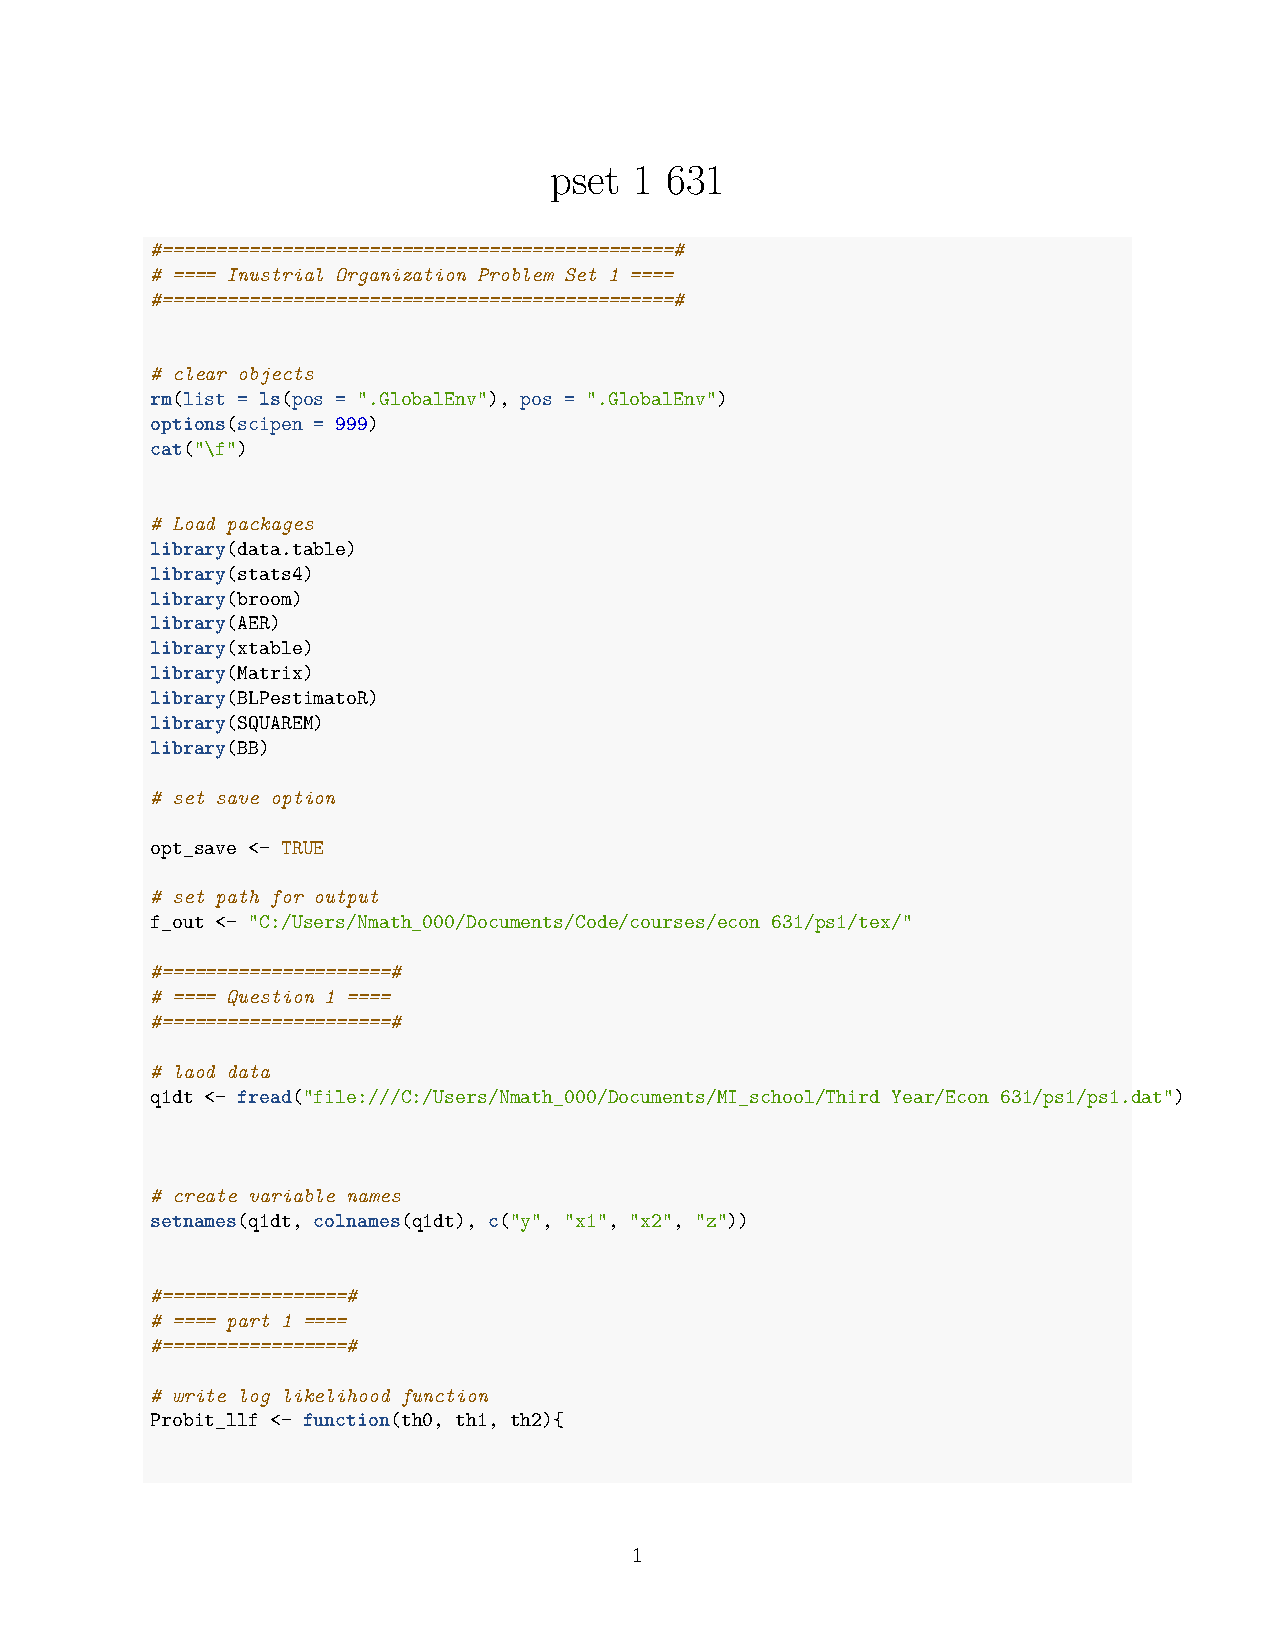
\includepdf[page=-]{assignment_1_r_code_pdf}




%------------------------------------------------
% end doc
%------------------------------------------------

\end{document}

